
%%%%%%%%%%%%%%%%%%%%%%%%%%%%%%%%%%%%%%%%%%%%%%%%%%%%%%%

\documentclass{iitthesis}
% \documentclass[draft]{iitthesis}

% Document Options:
%
% Note if you want to save paper when printing drafts,
% replace the above line by
%
%   \documentclass[draft]{iitthesis}
%
% See Help file for more about options.

\usepackage[dvips]{graphicx}    % This package is used for Figures
\usepackage{rotating}           % This package is used for landscape mode.
\usepackage{epsfig}
\usepackage{subfigure}          % These two packages, epsfig and subfigure, are used for creating subplots.
% Packages are explained in the Help document.


\begin{document}

%%% Declarations for Title Page %%%
\title{Title}
\author{Ozlem Kalinli}
\degree{Master of Science}
\dept{Electrical Engineering}
\date{May 2003}
\copyrightnoticetrue      % crate copyright page or not
%\coadvisortrue           % add co-advisor. activate it by removing % symbol to add co-advisor
\maketitle                % create title and copyright pages


\prelimpages         % Settings of preliminary pages are done with \prelimpages command


%%%  Acknowledgement %%%
\begin{acknowledgement}     % acknowledgement environment, this is optional
\par  This dissertation could not have been written without Dr. X
who not only served as my supervisor but also encouraged and
challenged me throughout my academic program. He and the other
faculty members, Dr. Y and Dr. Z, guided me through the
dissertation process, never accepting less than my best efforts. I
thank them all.\\ \\ (Don't copy this sample text. Write your own
acknowledgement.)
% or \input{acknowledgement.tex} % you need a separate acknowledgement.tex file to include it.
\end{acknowledgement}


% Table of Contents
\tableofcontents
\clearpage

% List of Tables
\listoftables

\clearpage

%List of Figures
\listoffigures

\clearpage

%List of Symbols(optional)

\listofsymbols
 \SymbolDefinition{$\beta$}{probability of non-detecting bad data}
 \SymbolDefinition{$\delta$}{Transition Coefficient Constant for the Design of Linear-Phase FIR Filters}
 \SymbolDefinition{$\zeta$}{Reflection Coefficient Parameter}


 \clearpage



%%% Abstract %%%
\begin{abstract}           % abstract environment, this is optional
\par Your Abstract goes here!
% or  This thesis investigates how to solve univariate integration problems using numerical methods, including the trapezoidal rule and the Simpson's rule. Most existing guaranteed algorithms are not adaptive and require too much a priori information. Most existing adaptive algorithms do not have valid justification for their results. The goal is to create adaptive algorithms utilizing the two above-mentioned methods with guarantees. The classes of integrands studied in this thesis are cones. The algorithms are analytically proved to be a success if the integrand lies in the cone. The algorithms are adaptive and automatically adjust the computational costs based on the integrand values. The lower and upper bounds on the computational costs for both algorithms are derived. The lower bounds on the complexity of the problems are derived as well. By comparing the upper bounds on the computational cost and the lower bounds on the complexity, our algorithms are shown to be asymptotically optimal. Numerical experiments are implemented.   %you need a separate abstract.tex file to include it.
\end{abstract}


\textpages     % Settings of text-pages are done with \textpages command

% Chapters are created with \Chapter{title} command
\Chapter{INTRODUCTION}

% Section are created with \Section{title} command
\Section{Basic Models} \label{sec:int}

In this chapter, we discuss the system identification problem for
discrete-time nonlinear dynamic systems. The discussion includes
an overview of the representations of various nonlinear systems
and their identification methods. Even though some of these
methods are developed for continuous-time system representations,
we only consider to work on the discrete-time representation of
the nonlinear systems. These techniques will guide us to develop
the FPET model structure. The main system equation we use here is:
% Equation Example1
\begin{equation}
 x^2+y^2 = z^2
 \label{eq:sample}   % is used to refer this equation in the text
\end{equation}
However, we will also represent a brief discuss on some more
complex cases as well.

\Section{Functional Series Methods in Linear Systems using Impulse
Response Generalization Algorithm}

One can represent a linear system by its impulse response.
Volterra developed a generalization of this representation for
nonlinear systems in which the single impulse response is replaced
with a series of integration kernels. This generalization of the
impulse response, usually called Volterra series, can be used to
approximate a wide variety of systems. For instance, Boyd and Chua
in \cite{HK}\footnote{Corresponding to references in the
Bibliography.} showed that a finite Volterra series can be used to
approximate any nonlinear operator which has fading memory. This
is explained in Section \ref{sec:int}. Now you will see a listing
example:
% An example for enumerate
\begin{enumerate}
  \item Suppression of hepatic glucose production
  \item Stimulation of hepatic glucose uptake
  \item Stimulation of glucose uptake by peripheral tissues,
  mainly muscle
\end{enumerate}

Fading memory concept can be defined as the effect of past inputs
on the present output fades out when time approaches infinity
\cite{Pan}. In general, we can write the input-output relationship
of any causal, discrete-time, time-invariant nonlinear systems by
a series of generalized convolutions \cite{MG}. Now you will see a
quotation example:

% A quotation example
% Every quota must be accompanied by a reference to the source
% in a footnote or in the Bibliography
\begin{quotation}
(This is a test for quotation environment!) In the Minimum
Variance Method, the peaks are sharp. We compare the graphs where
N=512 and p=64 and N=512 and p=128, it can be seen that when the
order p is increased frequency \cite{Boney96}.
\end{quotation}

\Subsection{Least Squares Based Identification} Block oriented
nonlinear systems can be represented by an interconnection of
linear dynamic and static nonlinear blocks. Well known block
oriented nonlinear models are Hammerstein, Wiener, and LNL
(Linear-Nonlinear-Linear) models as shown in the figure.
Hammerstein (NL, Nonlinear-Linear) and Wiener (LN,
Linear-Nonlinear) models are two special cases of the LNL cascade
model.You can see the results in Table \ref{table:nonlin}.


% Table Example1
\begin{table}[ht]
\caption{Nonlinear Model Results}   % title of Table
\centering                          % used for centering table
\begin{tabular}{c c c c}            % centered columns (4 columns)
\hline\hline                        % inserts double horizontal lines
Case & Method\#1 & Method\#2 & Method\#3 \\ [0.5ex] % inserts table heading
\hline                              % inserts single horizontal line below heading
1 & 50 & 837 & 970  \\              % inserting the body of the table
2 & 47 & 877 & 230  \\
3 & 31 & 25  & 415  \\
4 & 35 & 144 & 2356 \\
5 & 45 & 300 & 556 \\ [1ex]         % [1ex] adds vertical space
\hline                              % inserts single line
\end{tabular}
\label{table:nonlin}                % is used to refer this table in the text
\end{table}

% Table Example2
 \begin{table}[h]
 \caption{Performance Analysis using Hard Decision Detection Method in Low-Level Noise Systems with Nonlinear Behavior} % title of the table
 \centering                          % centering table
 \begin{tabular}{c rrrrrrr}          % creating eight columns
 \hline\hline                        % inserting double-line
 Audio Name&\multicolumn{7}{c}{Sum of Extracted Bits} \\ [0.5ex]
 \hline                                      % inserts single-line
 Police   & 5 & -1 &  5& 5& -7& -5& 3\\      % Entering row contents
 Midnight & 7 & -3 &  5& 3& -1& -3& 5\\
 News     & 9 & -3 &  7& 9& -5& -1& 9\\[1ex] % [1ex] adds vertical space
 \hline                                       % inserts single-line
 \end{tabular}
 \label{tab:hresult}
 \end{table}


% Figure Example1
% An example to show how to create a figure with LaTeX commands
\begin{figure}[h]
\setlength{\unitlength}{0.14in}     % selecting unit length
\centering                          % used for centering Figure
\begin{picture}(32,15)              % picture environment with the size (dimensions)
                                    % 32 length units wide, and 15 units high.
\put(3,4){\framebox(6,3){$H_{B}(q)$}}
\put(13,4){\framebox(6,3){$N[\cdot]$}}
\put(23,4){\framebox(6,3){$H_{C}(q)$}}
\put(0,5.5){\vector(1,0){3}}\put(9,5.5){\vector(1,0){4}}
\put(19,5.5){\vector(1,0){4}}\put(29,5.5){\vector(1,0){3}}
\put(-1,6.5) {$u(k)$}\put(30,6.5) {$y(k)$} \put(9.5,6.5)
{$x_{B}(k)$}\put(19.5,6.5) {$x_{C}(k)$}
\end{picture}
\caption{An LNL Block Oriented Model Structure}   % caption of the Figure
\label{fig:lnlblock}                              % label to refer this figure in text
\end{figure}


% Subsubsection is created using \Subsubsection{title} command, and text is
% typed in the same line.

\Subsubsection{Modified Periodogram} In the Modified Periodogram,
the spectrum is smoother and noise level is a little bit less
comparing to the Peridogram Method, since the data  is multiplied
with Hamming window. In the Bartlett Method, overlapping is not
used and K= 4. In this realization, we can see that frequency
resolution has been decreased (peaks are broader) .On the other
hand,noise level has been also reduced. As we expected, there is a
trade-off between frequency resolution and noise level. Decreasing
noise level is paid off by decreasing frequency resolution. In the
Blackman-Tuckey Method, both frequency resolution and noise level
seems good, see Figure \ref{fig:lnlblock}.

\Subsubsection{Other Useful Methods} There are some other methods
which are more complex for implementation. However, they will give
more efficient results. The figures below illustrate the results
obtained using method XYZ for a fuel metabolism process.

% Figure Example2
% An Example for importing an eps file
\begin{figure}[ht]
  \centering                % centering figure
  \scalebox{0.5}            % rescale the figure by a factor of 0.8
  {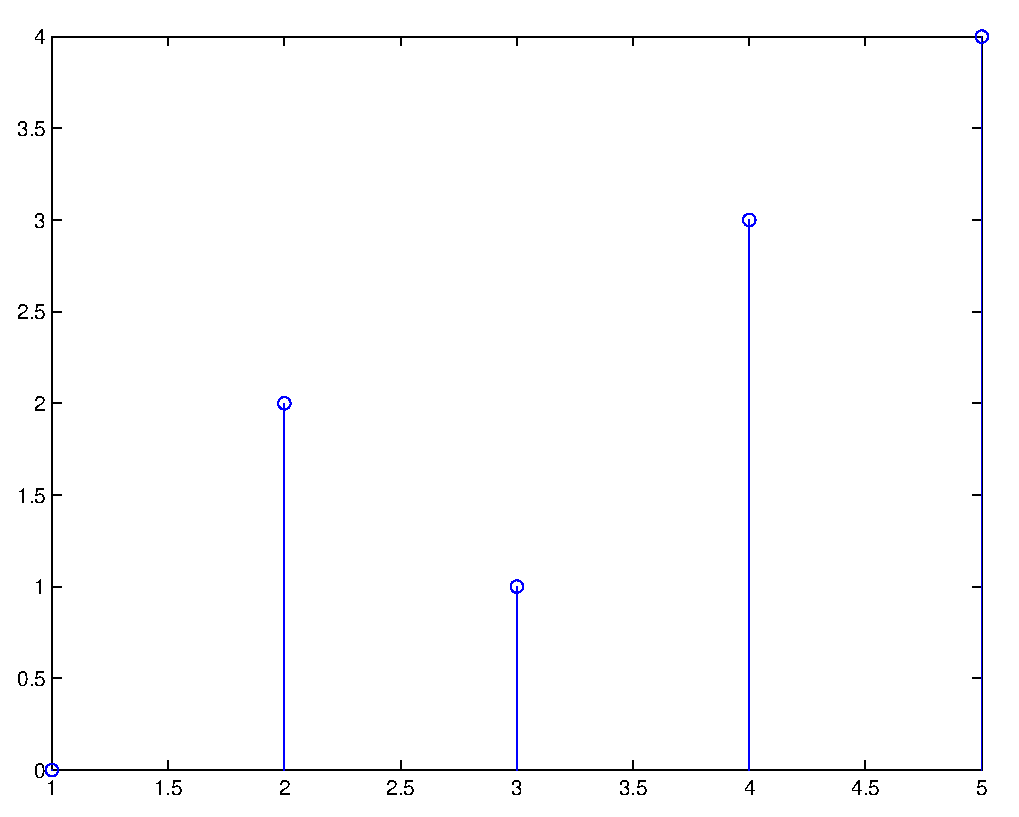
\includegraphics{matlab.ps}}   % importing figure
  \caption{Fuel Metabolism results with Method A}        % title of figure
  \label{fig:exm}                  % labelling to refer it inside the text
\end{figure}


% Figure Example5
% Creating subfigures
\begin{figure}[h]
 \vspace{10pt}
   \centering
 \mbox{\subfigure[Big]{\epsfig{figure=matlab.ps,width=3in}}\quad
       \subfigure[Small]{\epsfig{figure=matlab.ps,width=2in}}}
 \caption{Fuel Metabolism results using Method XYZ in complex systems for both linear and Nonlinear behavior cases}
 \label{fig:SubF}
 \end{figure}


\clearpage

\Chapter{Representation of Linear Constraints Methods with Convex
Function conditions in Modern Optimization Theory }

\Section{Basic Concepts}

In this chapter we examine ways of representing linear
constraints. The goal is to write the constraints in a form that
makes it easy to move from one feasible point to another. The
constraints specify interrelationship among the variables so that,
for example, if we increase the first variable, retaining
feasibility might require making a complicated sequence of changes
to all the other variables. It is much easier if we express the
constraints using a coordinate system that is "natural" for the
constraints. \footnote{Natural means that the points be global
optimums} Then the interrelationship among the variables are taken
care of by the coordinate system, and moves between feasible
points.

\Section{Null and Range Spaces}

The null sapce of a matrix is orthogonal to the rows of that
matrix......

\Section{Generating Null Space Matrices using VR Method}

VR stands for Variable Reduction method. This is a simple method
used in linear programming ......

\Section{Orthogonal Projection Matrix}

A matrix is called orthogonal projection if we have .......

\Chapter{Duality and Sensivity}

\Section{The Dual Problem}

For every linear programming problem there is a companion problem,
called dual linear problem...........

\Section{Duality Theory}

There are two major results relating the primal and dual problems.
The first is called weak duality and is easier to prove.

\Chapter{Network Problems}

\Section{Basic Examples}

The most general network problem that we face with is called  the
minimum cost network flow problem.

\Section{Basis Representation} Many of the efficiencies in the
network simplex method come about because of the special form of
the basis in the network problem.


\Chapter{CONCLUSION}
 %   \input{Conclusion.tex}
 You need a Conclusion.tex file


\Section{Summary}

This was just to create a sample section...

\clearpage


%
% APPENDIX
%

% Do the settings of appendices with \appendix command
\appendix

% Then create each appendix using
% \Appendix{title_of_appendix} command

\Appendix{Table of Transition Coefficients for the Design of
Linear-Phase FIR Filters}

Your Appendix will go here !

 \moretox

  \Appendix{Name of your Second
Appendix}

Your second appendix text....

\Appendix{Name of your Third Appendix}

Your third appendix text....
%
% BIBLIOGRAPHY
%
% you have two options: 1) create bibliography manually,
% 2) create bibliography automatically. See BibliographyHelp.pdf file for details.


\bibliographystyle{plain}
\bibliography{mybib}

\end{document}  % end of document
